% Options for packages loaded elsewhere
\PassOptionsToPackage{unicode}{hyperref}
\PassOptionsToPackage{hyphens}{url}
%
\documentclass[
]{article}
\usepackage{lmodern}
\usepackage{amssymb,amsmath}
\usepackage{ifxetex,ifluatex}
\ifnum 0\ifxetex 1\fi\ifluatex 1\fi=0 % if pdftex
  \usepackage[T1]{fontenc}
  \usepackage[utf8]{inputenc}
  \usepackage{textcomp} % provide euro and other symbols
\else % if luatex or xetex
  \usepackage{unicode-math}
  \defaultfontfeatures{Scale=MatchLowercase}
  \defaultfontfeatures[\rmfamily]{Ligatures=TeX,Scale=1}
\fi
% Use upquote if available, for straight quotes in verbatim environments
\IfFileExists{upquote.sty}{\usepackage{upquote}}{}
\IfFileExists{microtype.sty}{% use microtype if available
  \usepackage[]{microtype}
  \UseMicrotypeSet[protrusion]{basicmath} % disable protrusion for tt fonts
}{}
\makeatletter
\@ifundefined{KOMAClassName}{% if non-KOMA class
  \IfFileExists{parskip.sty}{%
    \usepackage{parskip}
  }{% else
    \setlength{\parindent}{0pt}
    \setlength{\parskip}{6pt plus 2pt minus 1pt}}
}{% if KOMA class
  \KOMAoptions{parskip=half}}
\makeatother
\usepackage{xcolor}
\IfFileExists{xurl.sty}{\usepackage{xurl}}{} % add URL line breaks if available
\IfFileExists{bookmark.sty}{\usepackage{bookmark}}{\usepackage{hyperref}}
\hypersetup{
  pdftitle={The effect of mRNA Vaccination on Small Gestational Age},
  pdfauthor={Busenur Kızılaslan},
  hidelinks,
  pdfcreator={LaTeX via pandoc}}
\urlstyle{same} % disable monospaced font for URLs
\usepackage[margin=1in]{geometry}
\usepackage{color}
\usepackage{fancyvrb}
\newcommand{\VerbBar}{|}
\newcommand{\VERB}{\Verb[commandchars=\\\{\}]}
\DefineVerbatimEnvironment{Highlighting}{Verbatim}{commandchars=\\\{\}}
% Add ',fontsize=\small' for more characters per line
\usepackage{framed}
\definecolor{shadecolor}{RGB}{248,248,248}
\newenvironment{Shaded}{\begin{snugshade}}{\end{snugshade}}
\newcommand{\AlertTok}[1]{\textcolor[rgb]{0.94,0.16,0.16}{#1}}
\newcommand{\AnnotationTok}[1]{\textcolor[rgb]{0.56,0.35,0.01}{\textbf{\textit{#1}}}}
\newcommand{\AttributeTok}[1]{\textcolor[rgb]{0.77,0.63,0.00}{#1}}
\newcommand{\BaseNTok}[1]{\textcolor[rgb]{0.00,0.00,0.81}{#1}}
\newcommand{\BuiltInTok}[1]{#1}
\newcommand{\CharTok}[1]{\textcolor[rgb]{0.31,0.60,0.02}{#1}}
\newcommand{\CommentTok}[1]{\textcolor[rgb]{0.56,0.35,0.01}{\textit{#1}}}
\newcommand{\CommentVarTok}[1]{\textcolor[rgb]{0.56,0.35,0.01}{\textbf{\textit{#1}}}}
\newcommand{\ConstantTok}[1]{\textcolor[rgb]{0.00,0.00,0.00}{#1}}
\newcommand{\ControlFlowTok}[1]{\textcolor[rgb]{0.13,0.29,0.53}{\textbf{#1}}}
\newcommand{\DataTypeTok}[1]{\textcolor[rgb]{0.13,0.29,0.53}{#1}}
\newcommand{\DecValTok}[1]{\textcolor[rgb]{0.00,0.00,0.81}{#1}}
\newcommand{\DocumentationTok}[1]{\textcolor[rgb]{0.56,0.35,0.01}{\textbf{\textit{#1}}}}
\newcommand{\ErrorTok}[1]{\textcolor[rgb]{0.64,0.00,0.00}{\textbf{#1}}}
\newcommand{\ExtensionTok}[1]{#1}
\newcommand{\FloatTok}[1]{\textcolor[rgb]{0.00,0.00,0.81}{#1}}
\newcommand{\FunctionTok}[1]{\textcolor[rgb]{0.00,0.00,0.00}{#1}}
\newcommand{\ImportTok}[1]{#1}
\newcommand{\InformationTok}[1]{\textcolor[rgb]{0.56,0.35,0.01}{\textbf{\textit{#1}}}}
\newcommand{\KeywordTok}[1]{\textcolor[rgb]{0.13,0.29,0.53}{\textbf{#1}}}
\newcommand{\NormalTok}[1]{#1}
\newcommand{\OperatorTok}[1]{\textcolor[rgb]{0.81,0.36,0.00}{\textbf{#1}}}
\newcommand{\OtherTok}[1]{\textcolor[rgb]{0.56,0.35,0.01}{#1}}
\newcommand{\PreprocessorTok}[1]{\textcolor[rgb]{0.56,0.35,0.01}{\textit{#1}}}
\newcommand{\RegionMarkerTok}[1]{#1}
\newcommand{\SpecialCharTok}[1]{\textcolor[rgb]{0.00,0.00,0.00}{#1}}
\newcommand{\SpecialStringTok}[1]{\textcolor[rgb]{0.31,0.60,0.02}{#1}}
\newcommand{\StringTok}[1]{\textcolor[rgb]{0.31,0.60,0.02}{#1}}
\newcommand{\VariableTok}[1]{\textcolor[rgb]{0.00,0.00,0.00}{#1}}
\newcommand{\VerbatimStringTok}[1]{\textcolor[rgb]{0.31,0.60,0.02}{#1}}
\newcommand{\WarningTok}[1]{\textcolor[rgb]{0.56,0.35,0.01}{\textbf{\textit{#1}}}}
\usepackage{graphicx,grffile}
\makeatletter
\def\maxwidth{\ifdim\Gin@nat@width>\linewidth\linewidth\else\Gin@nat@width\fi}
\def\maxheight{\ifdim\Gin@nat@height>\textheight\textheight\else\Gin@nat@height\fi}
\makeatother
% Scale images if necessary, so that they will not overflow the page
% margins by default, and it is still possible to overwrite the defaults
% using explicit options in \includegraphics[width, height, ...]{}
\setkeys{Gin}{width=\maxwidth,height=\maxheight,keepaspectratio}
% Set default figure placement to htbp
\makeatletter
\def\fps@figure{htbp}
\makeatother
\setlength{\emergencystretch}{3em} % prevent overfull lines
\providecommand{\tightlist}{%
  \setlength{\itemsep}{0pt}\setlength{\parskip}{0pt}}
\setcounter{secnumdepth}{-\maxdimen} % remove section numbering
\usepackage{booktabs}
\usepackage{longtable}
\usepackage{array}
\usepackage{multirow}
\usepackage{wrapfig}
\usepackage{float}
\usepackage{colortbl}
\usepackage{pdflscape}
\usepackage{tabu}
\usepackage{threeparttable}
\usepackage{threeparttablex}
\usepackage[normalem]{ulem}
\usepackage{makecell}
\usepackage{xcolor}

\title{\textbf{The effect of mRNA Vaccination on Small Gestational Age}}
\usepackage{etoolbox}
\makeatletter
\providecommand{\subtitle}[1]{% add subtitle to \maketitle
  \apptocmd{\@title}{\par {\large #1 \par}}{}{}
}
\makeatother
\subtitle{\textbf{\emph{Test Report}}}
\author{Busenur Kızılaslan}
\date{}

\begin{document}
\maketitle

{
\setcounter{tocdepth}{2}
\tableofcontents
}
\begin{Shaded}
\begin{Highlighting}[]
\NormalTok{The aim is to examine whether administration at least one dose of the mRNA-based vaccine in pregnancy is associated with shorter gestational age at birth. }
\end{Highlighting}
\end{Shaded}

\hypertarget{data-summary}{%
\section{Data Summary}\label{data-summary}}

\textbf{Garbage in, garbage out!}

The most important thing is to understand what is the data structure, in
this manner we need to ask a lot of questions to the data set.

\begin{itemize}
\item
  Is the data properly defined?
\item
  Are there any outliers and missing observations?
\end{itemize}

The data set has 12590 observations and 20 variables. All variables are
entered as numeric variables.

\begin{verbatim}
## 'data.frame':    12590 obs. of  20 variables:
##  $ pin                         : num  1 2 3 4 5 6 7 8 9 10 ...
##  $ vaccination                 : num  0 0 0 0 0 0 0 0 0 0 ...
##  $ gestationalweekofvaccination: num  NA NA NA NA NA NA NA NA NA NA ...
##  $ sarscov2_infection          : num  0 1 1 0 0 0 0 0 0 1 ...
##  $ ibu_prepreg                 : num  0 0 0 0 0 0 0 0 0 0 ...
##  $ paracet_prepreg             : num  1 1 1 1 1 1 1 1 1 0 ...
##  $ opioid_prepreg              : num  0 0 0 0 1 0 0 0 0 0 ...
##  $ diabetes                    : num  0 1 1 0 0 0 0 0 0 1 ...
##  $ depression_severity         : num  6 5.9 5.2 5.4 4.6 ...
##  $ pain                        : num  0 0 0 1 0 0 0 0 0 0 ...
##  $ headache                    : num  0 0 0 1 0 0 0 1 1 1 ...
##  $ pelvicgirdlepain            : num  0 1 0 0 1 0 1 1 1 0 ...
##  $ smoking                     : num  0 NA 0 0 0 0 0 0 0 0 ...
##  $ bmipp                       : num  25.4 33.1 27.9 25.6 20.8 ...
##  $ age                         : num  33.5 32.3 34.3 32.1 32 ...
##  $ parity                      : num  0 1 0 1 0 1 0 1 1 1 ...
##  $ education                   : num  1 1 0 1 1 1 0 1 0 1 ...
##  $ birthweight                 : num  4195 4001 4908 3697 4064 ...
##  $ gestage                     : num  266 280 260 281 269 ...
##  $ malform                     : num  0 0 0 0 0 0 0 0 0 0 ...
\end{verbatim}

Factor variables are fixed for the reliable analysis. Also, the data set
has possible outliers and missing values that have to be examined.

\begin{verbatim}
## 'data.frame':    12590 obs. of  20 variables:
##  $ pin                         : num  1 2 3 4 5 6 7 8 9 10 ...
##  $ vaccination                 : Factor w/ 2 levels "0","1": 1 1 1 1 1 1 1 1 1 1 ...
##  $ gestationalweekofvaccination: num  NA NA NA NA NA NA NA NA NA NA ...
##  $ sarscov2_infection          : Factor w/ 2 levels "0","1": 1 2 2 1 1 1 1 1 1 2 ...
##  $ ibu_prepreg                 : Factor w/ 2 levels "0","1": 1 1 1 1 1 1 1 1 1 1 ...
##  $ paracet_prepreg             : Factor w/ 2 levels "0","1": 2 2 2 2 2 2 2 2 2 1 ...
##  $ opioid_prepreg              : Factor w/ 2 levels "0","1": 1 1 1 1 2 1 1 1 1 1 ...
##  $ diabetes                    : Factor w/ 2 levels "0","1": 1 2 2 1 1 1 1 1 1 2 ...
##  $ depression_severity         : num  6 5.9 5.2 5.4 4.6 ...
##  $ pain                        : Factor w/ 2 levels "0","1": 1 1 1 2 1 1 1 1 1 1 ...
##  $ headache                    : Factor w/ 2 levels "0","1": 1 1 1 2 1 1 1 2 2 2 ...
##  $ pelvicgirdlepain            : Factor w/ 2 levels "0","1": 1 2 1 1 2 1 2 2 2 1 ...
##  $ smoking                     : Factor w/ 2 levels "0","1": 1 NA 1 1 1 1 1 1 1 1 ...
##  $ bmipp                       : num  25.4 33.1 27.9 25.6 20.8 ...
##  $ age                         : num  33.5 32.3 34.3 32.1 32 ...
##  $ parity                      : Factor w/ 2 levels "0","1": 1 2 1 2 1 2 1 2 2 2 ...
##  $ education                   : Factor w/ 2 levels "0","1": 2 2 1 2 2 2 1 2 1 2 ...
##  $ birthweight                 : num  4195 4001 4908 3697 4064 ...
##  $ gestage                     : num  266 280 260 281 269 ...
##  $ malform                     : Factor w/ 2 levels "0","1": 1 1 1 1 1 1 1 1 1 1 ...
\end{verbatim}

\hypertarget{outliers}{%
\subsection{Outliers}\label{outliers}}

Outliers can have many causes, such as: measurement or input error,
missing values, true outlier observation. There is no precise way to
define and identify outliers in general because of the specifics of each
dataset. Instead, researcher and an expert, must interpret the raw
observations and decide whether a value is an outlier or not. The data
set examined as univariate and multivariate perspective in order to
create a road map.

\hypertarget{univariate-outlier-evaluation}{%
\subsubsection{Univariate Outlier
Evaluation}\label{univariate-outlier-evaluation}}

Univariate outlier check is done with boxplot. It is seen that each
variable has outliers both upper and lower level. (\emph{This is an
interactive plot, you can add or exclude variables in a one click on
variable label, and you can see the points and thresholds on the plot})

\includegraphics{analyse_report_files/figure-latex/unnamed-chunk-5-1.pdf}

The outliers are examined. An observation can be observed as an outlier
in more than one variable. For this reason, the intersection must be
checked (7 intersecting observations were counted only once). Total
number of outliers are equal to 458, 23 of these observations belong to
the vaccinated observations. 435 of these observations belong to the
non-vaccinated observations.

At this point, the important question is \textbf{what is the rate of
vaccinated and non-vaccinated observations in the data?} The data set
has 207 vaccinated, and 12383 non-vaccinated observations. When we
compare each group within itself, it is seen that, in case of removing
outliers from the data set, 3.64\% of total observations are lost.
Although this rate is small, it is a significant loss because the rate
also equal to 11.11\% of vaccinated and 3.51\% of non-vaccinated
observations.

\hypertarget{multivariate-outlier-evaluation}{%
\subsubsection{Multivariate Outlier
Evaluation}\label{multivariate-outlier-evaluation}}

Multivariate outlier check is done by using spatial signs which is fast
algorithm for identifying multivariate outliers in high-dimensional
and/or large data sets. The computation of the distances is based on
Mahalanobis distances.

The data set has 295 possible outliers from multivariate perspective.
When we compare each group within itself, it is seen that, in case of
removing outliers from the data set, \%2.34 of total observations are
lost. They are equal to 1.45\% of vaccinated and 2.36\% of
non-vaccinated observations.

\hypertarget{decision}{%
\subsubsection{🎯 Decision}\label{decision}}

\textbf{The decision of which outliers to be eliminated should be made
together with the domain expert.} In this case study, the intersection
of outliers that is both univariate and multivariate possible outlier
set are selected as final outliers.

In the final case, 14 of outliers are eliminated which belong to
non-vaccinated observations.

\hypertarget{missing-values}{%
\subsection{Missing Values}\label{missing-values}}

After the outlier elimination, the missing values should be checked and
examined. It can be seen that, \(98.25\%\) of gestational week of
vaccination observation is missing. This rate also equal to the number
of non-vaccinated observations. As expected, a non-vaccinated
observation does not have a vaccination week information. For this
reason, gestational week of vaccination variable is excluded from the
data set before imputation.

\begin{wraptable}{r}{0pt}
\begin{tabular}[t]{l|r}
\hline
  & Missing Value(\%)\\
\hline
gestationalweekofvaccination & 98.2446386\\
\hline
depression\_severity & 0.5798253\\
\hline
smoking & 1.0722796\\
\hline
bmipp & 0.1191422\\
\hline
education & 0.2779984\\
\hline
gestage & 0.4289118\\
\hline
\end{tabular}\end{wraptable}

Under the assumption that data were missing at random (MAR), the missing
values are imputed. For imputation, Generates Multivariate Imputations
by Chained Equations (MICE) package is used that creates multiple
imputations for multivariate missing data. The method is based on Fully
Conditional Specification, where each incomplete variable is imputed by
a separate model. In this study, m is selected as 5 because the
substantive conclusions are unlikely to change as a result of raising m
beyond \(m=5\) (Van Buuren 2018).

In the beginning of imputation step, the data set is splitted into two
group which are vaccinated and non-vaccinated because of interactions.
Each group is imputed and then combined the imputed data sets (Van
Buuren 2018).

After the normality test, Bayesian linear regression is used for bmipp
and birthweight variables which are normally distributed. Predictive
mean matching is used for other variables for multiple imputation.

\begin{verbatim}
##               Test            Variable Statistic   p value Normality
## 1 Anderson-Darling depression_severity    5.9816  <0.001      NO    
## 2 Anderson-Darling        bmipp           0.7522  0.0503      YES   
## 3 Anderson-Darling         age            1.4548   9e-04      NO    
## 4 Anderson-Darling     birthweight        0.3083   0.56       YES   
## 5 Anderson-Darling       gestage          5.7090  <0.001      NO
\end{verbatim}

\hypertarget{decision-1}{%
\subsubsection{🎯 Decision}\label{decision-1}}

Except for the gestational week of vaccination variable, all missing
observations are imputed.

\hypertarget{data-modifications}{%
\subsection{Data Modifications}\label{data-modifications}}

In this study, the association between vaccine and small gestational age
at birth is examined. For this purpose, some of variables are converted
for usage and some new variables are created.

At this point, gestage (in days) values are converted from day to week.

\hypertarget{gestatinal-week-of-vaccination}{%
\subsubsection{Gestatinal Week of
Vaccination}\label{gestatinal-week-of-vaccination}}

As mentioned before, gestational week of vaccination variable has a lot
of missing value because the data set has a lot of non-vaccinated
observations. In order to use this important variable in the analysis
both vaccinated and non-vaccinated group, the continuous variable
converted to factor variable by using trimesters. This transformation
also provides ease of interpretation.

\begin{tabular}[t]{r|l|l}
\hline
value & trimesters & meaning\\
\hline
0 & NA & No vaccination\\
\hline
1 & 0 - 13 weeks & vaccination in 1st trimester\\
\hline
2 & 14 - 26 weeks & vaccination in 2nd trimester\\
\hline
3 & 27 - 40 weeks & vaccination in 3rd trimester\\
\hline
\end{tabular}

\hypertarget{determination-of-smallshort-gestational-age-sga}{%
\subsubsection{Determination of Small/Short Gestational Age
(SGA)}\label{determination-of-smallshort-gestational-age-sga}}

Small for gestational age (SGA) newborns are those who are smaller in
size than normal for the gestational age, most commonly defined as a
weight below the 10th percentile (threshold) for the gestational age
(MedlinePlus). In this study, SGA determination is done with the
proposed table (Talge et al. 2014). Thus, a new factor variable
gestatinal.age (\(SGA = 1\), \(AGA = 0\)) is generated using the
birthweight and gestage variables. Also, the variable gestage (in days)
is converted to week format for computational convenience.

\begin{verbatim}
## # A tibble: 23 x 2
##    GAweeks threshold
##      <int>     <dbl>
##  1      22       354
##  2      23       416
##  3      24       473
##  4      25       529
##  5      26       597
##  6      27       677
##  7      28       770
##  8      29       882
##  9      30      1018
## 10      31      1166
## # ... with 13 more rows
\end{verbatim}

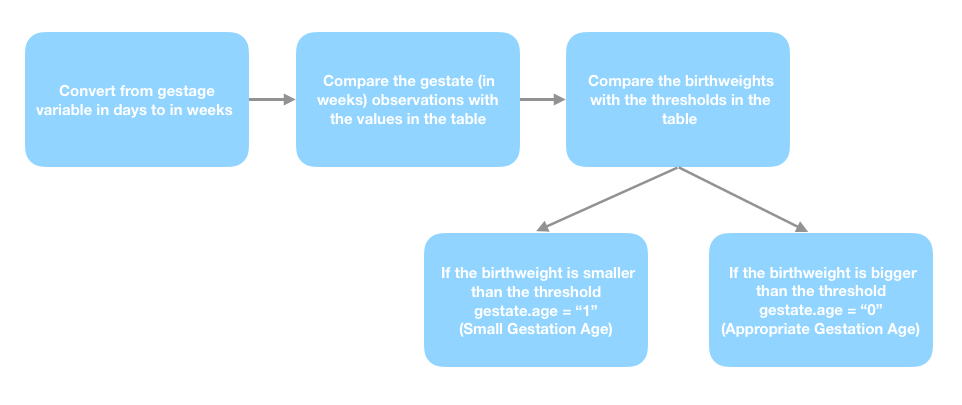
\includegraphics[width=1\linewidth]{table1}

\hypertarget{method}{%
\section{Method}\label{method}}

It is seen that, the vaccination variable has unbalanced groups as
vaccinated and non-vaccinated. For this reason, inverse probability of
treatment weighting (IPTW) is used to balance groups using a propensity
score matching weight approach.

The association between vaccine and small gestational age at birth is
examined with logistic regression because the gestational.age variable
is binary. In this manner, gestatinal.age and vaccination variables are
considered as response and explanatory variables, respectively. The
logistic regression is applied both before and after IPTW for comparison
purpose.

\hypertarget{the-summary-of-variables-beforeafter-inverse-probability-of-treatment-weighting-iptw}{%
\subsection{The Summary of Variables Before/After Inverse Probability of
Treatment Weighting
(IPTW)}\label{the-summary-of-variables-beforeafter-inverse-probability-of-treatment-weighting-iptw}}

In the IPTW method, the propensity score is defined as the probability
of being vaccinated. It is obtained from a logistic regression model
where the vaccination variable is considered as a binary dependent
variable and the following list of covariates is considered as the
independent variables.

\begin{verbatim}
##  [1] "ibu_prepreg"         "paracet_prepreg"     "opioid_prepreg"     
##  [4] "diabetes"            "depression_severity" "pain"               
##  [7] "headache"            "pelvicgirdlepain"    "smoking"            
## [10] "bmipp"               "age"                 "parity"             
## [13] "education"           "malform"             "sarscov2_infection"
\end{verbatim}

Balance before and after IPTW assessed using the standardized mean
difference (SMD) between vaccination groups. A SMD of greater that 0.1
is usually considered to indicate a significant imbalance(Austin 2009).

After the missing data imputation, 5 imputed data sets are obtained. In
the next, firstly, we present results for the first imputation data sets
(\(m = 1\)). Then, the combination of all imputed data set results are
presented.

Unweighted distribution of baseline characteristics of the study
population for \(m=1\).

\begin{verbatim}
##                                  Stratified by vaccination
##                                   0             1             SMD   
##   n                               12369           207               
##   ibu_prepreg = 1 (%)              3172 (25.6)     59 (28.5)   0.064
##   paracet_prepreg = 1 (%)         10310 (83.4)    176 (85.0)   0.046
##   opioid_prepreg = 1 (%)           1239 (10.0)     26 (12.6)   0.080
##   diabetes = 1 (%)                 1764 (14.3)     32 (15.5)   0.034
##   depression_severity (mean (SD))  4.99 (1.00)   5.70 (0.85)   0.762
##   pain = 1 (%)                      982 ( 7.9)     10 ( 4.8)   0.127
##   headache = 1 (%)                 3891 (31.5)     75 (36.2)   0.101
##   pelvicgirdlepain = 1 (%)         6798 (55.0)    113 (54.6)   0.007
##   smoking = 1 (%)                   749 ( 6.1)    180 (87.0)   2.772
##   bmipp (mean (SD))               26.49 (3.12)  26.19 (3.05)   0.099
##   age (mean (SD))                 32.09 (2.24)  32.00 (2.21)   0.039
##   parity = 1 (%)                   6218 (50.3)     69 (33.3)   0.349
##   education = 1 (%)                9269 (74.9)    152 (73.4)   0.034
##   malform = 1 (%)                   566 ( 4.6)     26 (12.6)   0.288
##   sarscov2_infection = 1 (%)        920 ( 7.4)      0 ( 0.0)   0.401
\end{verbatim}

It is concluded that 7 variables have a SMD of greater than 0.1.

\begin{verbatim}
##                        1 vs 2
## depression_severity 0.7620462
## pain                0.1273928
## headache            0.1010245
## smoking             2.7723626
## parity              0.3485737
## malform             0.2882136
## sarscov2_infection  0.4008899
\end{verbatim}

\hypertarget{propensity-score-estimation}{%
\subsection{Propensity Score
Estimation}\label{propensity-score-estimation}}

For \(m = 1\), IPTW performed for a set of the selected covariates using
the propensity score. Logistic regression is fitted to estimate the
probability of vaccination groups.

\begin{verbatim}
## 
## Call:  glm(formula = vaccination ~ ibu_prepreg + paracet_prepreg + opioid_prepreg + 
##     diabetes + depression_severity + pain + headache + pelvicgirdlepain + 
##     smoking + bmipp + age + parity + education + malform + sarscov2_infection, 
##     family = binomial(link = "logit"), data = merged.data.rev1)
## 
## Coefficients:
##         (Intercept)         ibu_prepreg1     paracet_prepreg1  
##          -12.495992             0.213107             0.162699  
##     opioid_prepreg1            diabetes1  depression_severity  
##            0.059400             1.271233             1.369380  
##               pain1            headache1    pelvicgirdlepain1  
##           -0.264455             0.188465            -0.110322  
##            smoking1                bmipp                  age  
##            4.973338            -0.020595            -0.007185  
##             parity1           education1             malform1  
##           -0.931643            -0.193988             0.001348  
## sarscov2_infection1  
##          -18.178769  
## 
## Degrees of Freedom: 12575 Total (i.e. Null);  12560 Residual
## Null Deviance:       2111 
## Residual Deviance: 1035  AIC: 1067
\end{verbatim}

\begin{verbatim}
## 
## Call:
## glm(formula = vaccination ~ ibu_prepreg + paracet_prepreg + opioid_prepreg + 
##     diabetes + depression_severity + pain + headache + pelvicgirdlepain + 
##     smoking + bmipp + age + parity + education + malform + sarscov2_infection, 
##     family = binomial(link = "logit"), data = merged.data.rev1)
## 
## Deviance Residuals: 
##     Min       1Q   Median       3Q      Max  
## -1.6360  -0.0782  -0.0448  -0.0245   4.1528  
## 
## Coefficients:
##                       Estimate Std. Error z value Pr(>|z|)    
## (Intercept)         -12.495992   1.616186  -7.732 1.06e-14 ***
## ibu_prepreg1          0.213107   0.191144   1.115    0.265    
## paracet_prepreg1      0.162699   0.237279   0.686    0.493    
## opioid_prepreg1       0.059400   0.261738   0.227    0.820    
## diabetes1             1.271233   0.278083   4.571 4.84e-06 ***
## depression_severity   1.369380   0.111083  12.328  < 2e-16 ***
## pain1                -0.264455   0.385929  -0.685    0.493    
## headache1             0.188465   0.179808   1.048    0.295    
## pelvicgirdlepain1    -0.110322   0.172889  -0.638    0.523    
## smoking1              4.973338   0.228490  21.766  < 2e-16 ***
## bmipp                -0.020595   0.026802  -0.768    0.442    
## age                  -0.007185   0.038240  -0.188    0.851    
## parity1              -0.931643   0.180559  -5.160 2.47e-07 ***
## education1           -0.193988   0.195619  -0.992    0.321    
## malform1              0.001348   0.275040   0.005    0.996    
## sarscov2_infection1 -18.178769 488.240139  -0.037    0.970    
## ---
## Signif. codes:  0 '***' 0.001 '**' 0.01 '*' 0.05 '.' 0.1 ' ' 1
## 
## (Dispersion parameter for binomial family taken to be 1)
## 
##     Null deviance: 2110.8  on 12575  degrees of freedom
## Residual deviance: 1034.7  on 12560  degrees of freedom
## AIC: 1066.7
## 
## Number of Fisher Scoring iterations: 19
\end{verbatim}

The matching weight method (Li and Greene 2013) is used for creating
weights. The matching weight is defined as the smaller of the predicted
probabilities of receiving or not receiving the treatment (vaccination)
over the predicted probability of being assigned to the patient is
actually in. After weighting, all the standardized mean differences are
below 0.1.

\begin{verbatim}
##                                  Stratified by vaccination
##                                   0              1              SMD   
##   n                                165.1          175.1               
##   ibu_prepreg = 1 (%)               46.7 (28.3)    48.0 (27.4)   0.020
##   paracet_prepreg = 1 (%)          138.1 (83.6)   148.2 (84.6)   0.027
##   opioid_prepreg = 1 (%)            20.6 (12.5)    21.8 (12.5)  <0.001
##   diabetes = 1 (%)                  22.7 (13.7)    19.9 (11.4)   0.071
##   depression_severity (mean (SD))   5.46 (0.84)    5.52 (0.76)   0.082
##   pain = 1 (%)                       7.2 ( 4.3)     8.7 ( 5.0)   0.029
##   headache = 1 (%)                  55.1 (33.4)    60.8 (34.7)   0.029
##   pelvicgirdlepain = 1 (%)          91.2 (55.3)    96.9 (55.3)   0.002
##   smoking = 1 (%)                  137.8 (83.5)   148.1 (84.6)   0.030
##   bmipp (mean (SD))                26.05 (3.36)   26.11 (3.07)   0.017
##   age (mean (SD))                  32.12 (2.32)   32.10 (2.18)   0.009
##   parity = 1 (%)                    59.2 (35.8)    61.3 (35.0)   0.018
##   education = 1 (%)                122.8 (74.4)   129.7 (74.1)   0.006
##   malform = 1 (%)                   19.9 (12.1)    21.1 (12.1)   0.001
##   sarscov2_infection = 1 (%)         0.0 ( 0.0)     0.0 ( 0.0)  <0.001
\end{verbatim}

In the next table and figure, after and before IPTW results of baseline
characteristics and SMD values of considered independent variables are
presented.

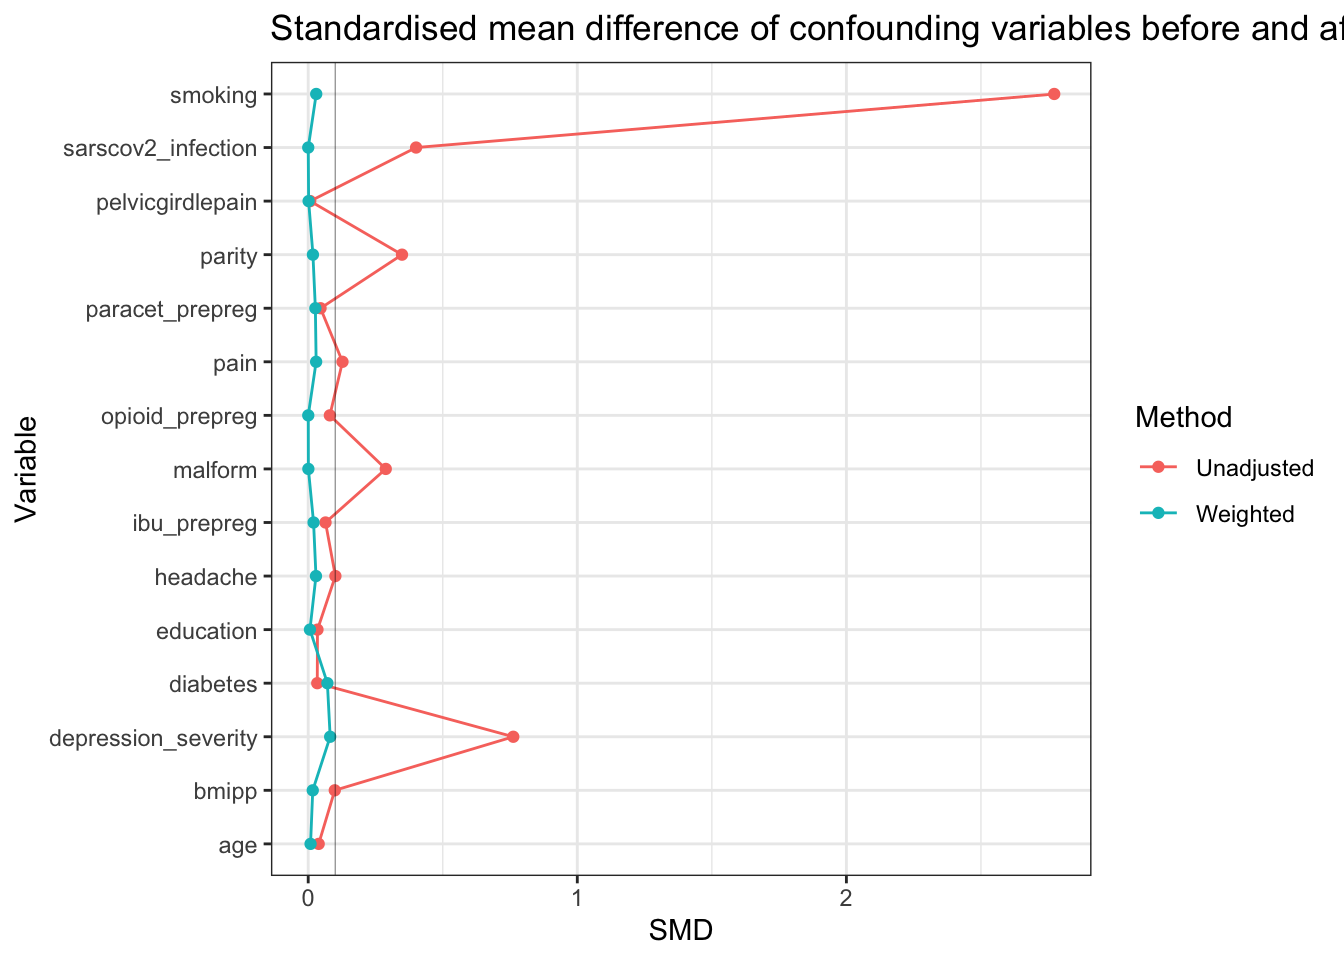
\includegraphics{analyse_report_files/figure-latex/unnamed-chunk-27-1.pdf}

\begin{verbatim}
##                                 Unweighted                         
## Group                           No Vaccination Vacination    SMD   
## n                               12369            207               
## ibu_prepreg = 1 (%)              3172 (25.6)      59 (28.5)   0.064
## paracet_prepreg = 1 (%)         10310 (83.4)     176 (85.0)   0.046
## opioid_prepreg = 1 (%)           1239 (10.0)      26 (12.6)   0.080
## diabetes = 1 (%)                 1764 (14.3)      32 (15.5)   0.034
## depression_severity (mean (SD))  4.99 (1.00)    5.70 (0.85)   0.762
## pain = 1 (%)                      982 ( 7.9)      10 ( 4.8)   0.127
## headache = 1 (%)                 3891 (31.5)      75 (36.2)   0.101
## pelvicgirdlepain = 1 (%)         6798 (55.0)     113 (54.6)   0.007
## smoking = 1 (%)                   749 ( 6.1)     180 (87.0)   2.772
## bmipp (mean (SD))               26.49 (3.12)   26.19 (3.05)   0.099
## age (mean (SD))                 32.09 (2.24)   32.00 (2.21)   0.039
## parity = 1 (%)                   6218 (50.3)      69 (33.3)   0.349
## education = 1 (%)                9269 (74.9)     152 (73.4)   0.034
## malform = 1 (%)                   566 ( 4.6)      26 (12.6)   0.288
## sarscov2_infection = 1 (%)        920 ( 7.4)       0 ( 0.0)   0.401
##                                 Weighted                            
## Group                           No Vaccination Vacination     SMD   
## n                                165.1          175.1               
## ibu_prepreg = 1 (%)               46.7 (28.3)    48.0 (27.4)   0.020
## paracet_prepreg = 1 (%)          138.1 (83.6)   148.2 (84.6)   0.027
## opioid_prepreg = 1 (%)            20.6 (12.5)    21.8 (12.5)  <0.001
## diabetes = 1 (%)                  22.7 (13.7)    19.9 (11.4)   0.071
## depression_severity (mean (SD))   5.46 (0.84)    5.52 (0.76)   0.082
## pain = 1 (%)                       7.2 ( 4.3)     8.7 ( 5.0)   0.029
## headache = 1 (%)                  55.1 (33.4)    60.8 (34.7)   0.029
## pelvicgirdlepain = 1 (%)          91.2 (55.3)    96.9 (55.3)   0.002
## smoking = 1 (%)                  137.8 (83.5)   148.1 (84.6)   0.030
## bmipp (mean (SD))                26.05 (3.36)   26.11 (3.07)   0.017
## age (mean (SD))                  32.12 (2.32)   32.10 (2.18)   0.009
## parity = 1 (%)                    59.2 (35.8)    61.3 (35.0)   0.018
## education = 1 (%)                122.8 (74.4)   129.7 (74.1)   0.006
## malform = 1 (%)                   19.9 (12.1)    21.1 (12.1)   0.001
## sarscov2_infection = 1 (%)         0.0 ( 0.0)     0.0 ( 0.0)  <0.001
\end{verbatim}

This analysis is conducted before and after IPTW for \(m = 1\). The
before IPTW results are given as follows.

\begin{verbatim}
## 
## Call:
## glm(formula = (gestational.age == 1) ~ vaccination, family = binomial(link = "logit"), 
##     data = merged.data.rev1)
## 
## Deviance Residuals: 
##     Min       1Q   Median       3Q      Max  
## -0.1709  -0.0685  -0.0685  -0.0685   3.4801  
## 
## Coefficients:
##              Estimate Std. Error z value Pr(>|z|)    
## (Intercept)   -6.0533     0.1859 -32.560  < 2e-16 ***
## vaccination1   1.8338     0.6106   3.003  0.00267 ** 
## ---
## Signif. codes:  0 '***' 0.001 '**' 0.01 '*' 0.05 '.' 0.1 ' ' 1
## 
## (Dispersion parameter for binomial family taken to be 1)
## 
##     Null deviance: 446.24  on 12575  degrees of freedom
## Residual deviance: 440.52  on 12574  degrees of freedom
## AIC: 444.52
## 
## Number of Fisher Scoring iterations: 9
\end{verbatim}

\begin{verbatim}
##  (Intercept) vaccination1 
##  0.002350081  6.257606491
\end{verbatim}

The after IPTW results are given as follows.

\begin{verbatim}
## 
## Call:
## glm(formula = (gestational.age == 1) ~ vaccination, family = quasibinomial(), 
##     data = merged.data.rev1, weights = ps_weights)
## 
## Deviance Residuals: 
##      Min        1Q    Median        3Q       Max  
## -0.17543  -0.00896  -0.00509  -0.00281   2.89200  
## 
## Coefficients:
##              Estimate Std. Error t value Pr(>|t|)    
## (Intercept)   -4.4077     0.1174 -37.544   <2e-16 ***
## vaccination1   0.2413     0.1551   1.556     0.12    
## ---
## Signif. codes:  0 '***' 0.001 '**' 0.01 '*' 0.05 '.' 0.1 ' ' 1
## 
## (Dispersion parameter for quasibinomial family taken to be 0.02705635)
## 
##     Null deviance: 49.253  on 12575  degrees of freedom
## Residual deviance: 49.187  on 12574  degrees of freedom
## AIC: NA
## 
## Number of Fisher Scoring iterations: 7
\end{verbatim}

\begin{verbatim}
##  (Intercept) vaccination1 
##   -4.4077260    0.2412678
\end{verbatim}

\begin{verbatim}
##  (Intercept) vaccination1 
##   0.01218285   1.27286190
\end{verbatim}

\hypertarget{final-analysis}{%
\subsection{Final Analysis}\label{final-analysis}}

In this part, the analysis conducted with all imputed data sets (m is
selected 5) after IPTW, and the results are combined with pool function.

In the next, the analysis conducted with all imputed data sets (m is
selected 5) after IPTW, and the results are combined with pool function.

\begin{Shaded}
\begin{Highlighting}[]
\NormalTok{ffit}\OperatorTok{$}\NormalTok{estimate }\OperatorTok\StringTok{ }\KeywordTok{exp}\NormalTok{()}
\end{Highlighting}
\end{Shaded}

\begin{verbatim}
## [1] 0.01208202 1.28640515
\end{verbatim}

\hypertarget{limitations}{%
\section{Limitations}\label{limitations}}

\begin{itemize}
\tightlist
\item
  vaccinated and unvaccinated observations are not equal.
\end{itemize}

\hypertarget{comments}{%
\section{Comments}\label{comments}}

Family-based studies showed that gestational age at birth is partially
(from 25\% to 40\%) determined by genetic factors (Clausson,
Lichtenstein, and Cnattingius 2000).

The ratio between fetal growth rate and uterine size (reflecting uterine
distension) is suspected to partially determine the pregnancy length
(Bacelis et al. 2018).

\hypertarget{ideas}{%
\section{🚀 Ideas}\label{ideas}}

\hypertarget{packages-and-details}{%
\section{Packages and Details}\label{packages-and-details}}

In this study, R statistical software(R Core Team 2022) (version 4.2.0)
is used. The interactive report is prepared with R Markdown. The
packages used in the study are listed below.

\begin{Shaded}
\begin{Highlighting}[]
\NormalTok{readr, tidyverse, magrittr, naniar, mice, dplyr, GGally, finalfit, usethis, devtools, psych, ltm, VIM, plotly, nortest, car, Hmisc, purrr, reshape2, MVN, mvoutlier,  kableExtra, grid, shadowtext,  tableone, Matching, survey, ggplot2}
\end{Highlighting}
\end{Shaded}

\hypertarget{references}{%
\section*{References}\label{references}}
\addcontentsline{toc}{section}{References}

\hypertarget{refs}{}
\leavevmode\hypertarget{ref-austin2009balance}{}%
Austin, Peter C. 2009. ``Balance Diagnostics for Comparing the
Distribution of Baseline Covariates Between Treatment Groups in
Propensity-Score Matched Samples.'' \emph{Statistics in Medicine} 28
(25): 3083--3107.

\leavevmode\hypertarget{ref-bacelis2018uterine}{}%
Bacelis, Jonas, Julius Juodakis, Kristina M Adams Waldorf, Verena
Sengpiel, Louis J Muglia, Ge Zhang, and Bo Jacobsson. 2018. ``Uterine
Distention as a Factor in Birth Timing: Retrospective Nationwide Cohort
Study in Sweden.'' \emph{BMJ Open} 8 (10): e022929.

\leavevmode\hypertarget{ref-clausson2000genetic}{}%
Clausson, Britt, Paul Lichtenstein, and Sven Cnattingius. 2000.
``Genetic Influence on Birthweight and Gestational Length Determined by
Studies in Offspring of Twins.'' \emph{BJOG: An International Journal of
Obstetrics \& Gynaecology} 107 (3): 375--81.

\leavevmode\hypertarget{ref-li2013weighting}{}%
Li, Liang, and Tom Greene. 2013. ``A Weighting Analogue to Pair Matching
in Propensity Score Analysis.'' \emph{The International Journal of
Biostatistics} 9 (2): 215--34.

\leavevmode\hypertarget{ref-r}{}%
R Core Team. 2022. \emph{R: A Language and Environment for Statistical
Computing}. Vienna, Austria: R Foundation for Statistical Computing.
\url{https://www.R-project.org/}.

\leavevmode\hypertarget{ref-talge2014united}{}%
Talge, Nicole M, Lanay M Mudd, Alla Sikorskii, and Olga Basso. 2014.
``United States Birth Weight Reference Corrected for Implausible
Gestational Age Estimates.'' \emph{Pediatrics} 133 (5): 844--53.

\leavevmode\hypertarget{ref-buuren}{}%
Van Buuren, S. 2018. \emph{Flexible Imputation of Missing Data}. CRC
press. \url{https://stefvanbuuren.name/fimd/}.

\end{document}
